\documentclass{beamer}
\usetheme{Madrid}
\usecolortheme{default}

\usepackage{graphicx}
\usepackage{booktabs}

\title[Configuration vs. Detector Class]{Configuration Still Beats Algorithm, Until the Drift Hides in the Correlations}
\subtitle{Extending Resource-Constrained Drift Detection to Multivariate Shift}
\author{Stephen Kwaku Azongo}
\institute{Department of Computer Science, University of Ghana}
\date{\today}

\begin{document}

\frame{\titlepage}

\begin{frame}{Motivation: Two Open Questions from Paper 1}
\begin{block}{Paper 1's finding}
Monitoring configuration (frequency, window size) beats detector algorithm choice, by a 37-fold margin in detection delay, for three univariate detectors.
\end{block}
\vspace{0.5em}
\textbf{Two questions that finding leaves open:}
\begin{enumerate}
  \item Does this survive extending to \textbf{genuinely multivariate} detectors?
  \item Rabanser et al.\ (2019, NeurIPS) found univariate testing \textbf{rivals} multivariate testing, on shifts that all move some feature's own distribution. What if a shift leaves \textbf{every marginal untouched}?
\end{enumerate}
\vspace{0.5em}
\begin{block}{This study}
Two experimental grids, one that extends Paper 1's condition to multivariate detectors, one built specifically so univariate testing \emph{cannot} succeed.
\end{block}
\end{frame}

\begin{frame}{Methodology}
\begin{columns}[T]
\begin{column}{0.5\textwidth}
\textbf{Same 3 datasets}, now with 2 correlated features each
\begin{itemize}
  \item Credit: AGE + BILL\_AMT1
  \item Telco: Monthly + Total Charges
  \item Maintenance: Tool wear + Air temp.
\end{itemize}
\textbf{6 detectors}
\begin{itemize}
  \item Univariate: KS, PSI, Wasserstein
  \item Multivariate: MMD, C2ST, HDDDM
\end{itemize}
\end{column}
\begin{column}{0.5\textwidth}
\textbf{Two drift conditions}
\begin{itemize}
  \item \textbf{Marginal}: shifts each feature's own distribution (16{,}200 runs)
  \item \textbf{Correlation-only}: rank-permutation, marginals provably unchanged (3{,}240 runs)
\end{itemize}
\end{column}
\end{columns}
\vspace{1em}
\begin{center}
\small Kruskal-Wallis, Mann-Whitney U, Spearman $\rho$, $\chi^2$, study-wide FDR correction
\end{center}
\end{frame}

\begin{frame}{Result 1: Configuration Dominance Replicates}
\begin{center}
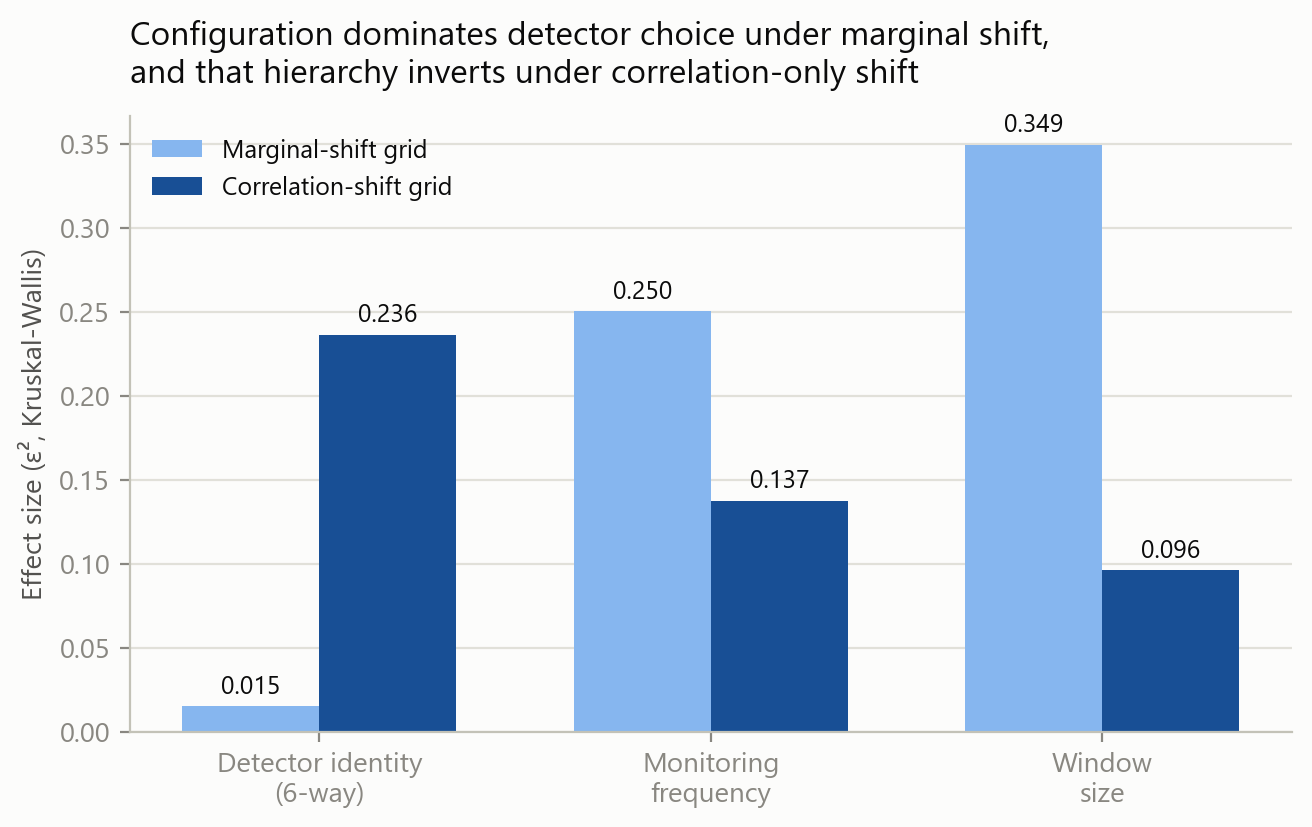
\includegraphics[width=0.58\textwidth]{figures/fig3_effect_size_hierarchy.png}
\end{center}
\begin{itemize}
  \item Marginal grid: window size $\varepsilon^2 = 0.349$ vs.\ detector identity $\varepsilon^2 = 0.015$
  \item Detector \textbf{class} has \emph{no} effect on whether drift is caught at all ($\chi^2$, $p=0.21$)
  \item Paper 1's finding holds under a harder, multivariate setting
\end{itemize}
\end{frame}

\begin{frame}{Result 2: The Hierarchy Inverts, Sharply}
\begin{center}
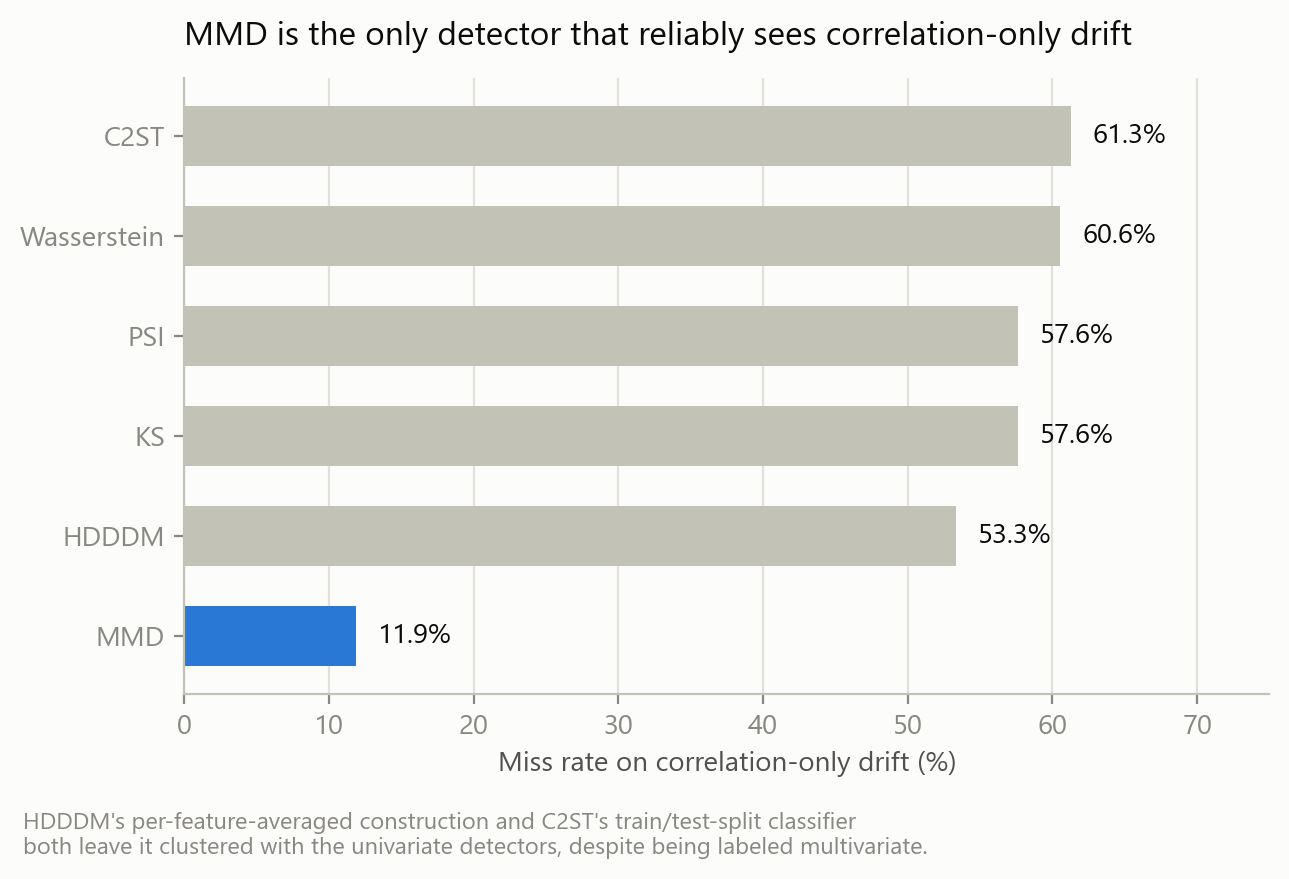
\includegraphics[width=0.68\textwidth]{figures/fig4_correlation_miss_rate_emphasis.png}
\end{center}
\begin{itemize}
  \item Correlation-only grid: detector identity $\varepsilon^2 = 0.236$, now \textbf{larger} than either constraint effect
  \item Whether drift is caught at all: $\chi^2=86.7$, $p=1.3\times10^{-20}$
\end{itemize}
\end{frame}

\begin{frame}{The Real Story: Construction, Not Class}
\begin{center}
\small
\begin{tabular}{lcc}
\toprule
Detector & Miss rate & Sees joint structure? \\
\midrule
MMD & 11.9\% & Yes, by kernel construction \\
HDDDM & 53.3\% & \textbf{No}: averages per-feature distances \\
C2ST & 61.3\% & In principle, but sample-starved \\
\bottomrule
\end{tabular}
\end{center}
\vspace{1em}
\begin{block}{The point}
HDDDM is labelled multivariate but its own published formula (Ditzler \& Polikar, 2011) mathematically cannot see correlation structure. The label doesn't predict performance; the statistic's construction does.
\end{block}
\end{frame}

\begin{frame}{Correlation-Only Drift: Easy to Catch, Mostly Benign}
\begin{center}
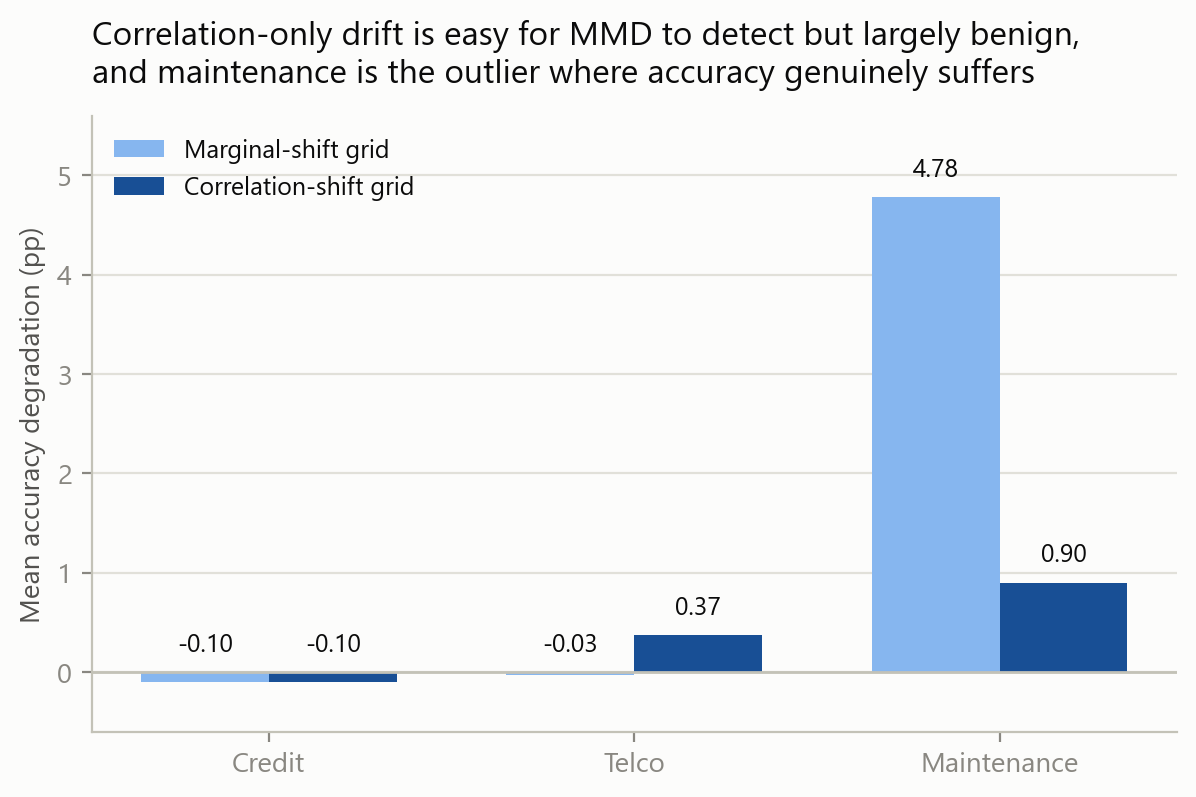
\includegraphics[width=0.58\textwidth]{figures/fig6_accuracy_degradation.png}
\end{center}
\begin{itemize}
  \item Maintenance is the outlier where accuracy genuinely suffers
  \item Credit and Telco: near-zero impact in both conditions
  \item Echoes Rabanser et al.'s distinction: detectable $\neq$ malignant
\end{itemize}
\end{frame}

\begin{frame}{Takeaways for Practitioners}
\begin{enumerate}
  \item \textbf{Configuration first}, still, whenever drift has a marginal signature
  \item If monitored features could drift \textbf{jointly} without moving individually: detector choice now matters most
  \item Don't trust the \textbf{multivariate label} alone: check whether the statistic actually uses cross-feature dependency
\end{enumerate}
\vspace{1em}
\begin{block}{Limitations}
Two-feature pairs only; single model (Random Forest); Wasserstein threshold empirically, not literature, calibrated; synthetic injection throughout
\end{block}
\begin{block}{Next steps}
Higher-dimensional feature groups; C2ST at larger windows; embedding-space extension (text/vision) as future work, not required here
\end{block}
\end{frame}

\end{document}
